\achapter{2}{The Matrix Representation of a Linear System} \label{sec:matrix_representation}


\vspace*{-17 pt}
\framebox{
\parbox{\dimexpr\linewidth-3\fboxsep-3\fboxrule}
{\begin{fqs}
\item What is a matrix?
\item How do we associate a matrix to a system of linear equations?
\item What row operations can we perform on an augmented matrix of a linear system to solve the system of linear equations?
\item What are pivots, basic variables, and free variables? 
\item How many solutions can a system of linear equations have?
\item When is a linear system consistent?
\item When does a linear system have infinitely many solutions? A unique solution?
\item How can we represent the set of solutions to a consistent system if the system has infinitely many solutions?
\end{fqs}}}% \hspace*{3 pt}}

\vspace*{13 pt}

\csection{Application: Approximating Area Under a Curve}

We know from basic geometry how to find areas of circles and triangles. However, it is much more difficult to find areas of other geometric objects. In fact, it is generally an impossible problem to determine the exact area bounded by a complicated curve. For this reason, approximation methods are used. One such method involves approximating curves using quadratic functions.

Unless you have learned some calculus, you have probably never calculated the area under a parabola. In the ancient work \emph{Quadrature of the Parabola} (3rd century BC), Archimedes determined a method for finding the area of a region bounded by a parabola by using mechanics and then by geometric methods. Once we know how to calculate the area of a region bounded by a parabola, Simpson's Rule uses parabolas to approximate a function, and then approximates the area under the graph of the graph of the function by using the areas under the parabolas. In order to use Simpsons Rule, we need to know how to exactly fit a quadratic function to three points. More details about this process can be found at the end of this section. This idea of fitting a polynomial to a set of data points has uses in other areas as well. For example, two common applications of B\'{e}zier curves are font design and drawing tools. When fitting a polynomial to a large set of data points, our systems of equations can become quite large, and can be difficult to solve by hand.  In this section we will see how to use matrices to more conveniently represent systems of equations of any size. We also consider how the elimination process works on the matrix representation of a linear system and how we can determine the existence of solutions and the form of solutions of a linear system.

\csection{Introduction}

When working with a linear system, the labels for the variables are irrelevant to the solution -- the only thing that matters is the coefficients of the variables in the equations and the constants on the other side of the equations. For example, given a linear system of the form

\begin{equation}  \label{eq:PA_1}
\begin{alignedat}{4}
a_2 	&{}-{} 	&a_1 	&{}+{}	&a_0 &= 2 \\
a_2 	&{}+{} 	&a_1 	&{}+{} 	&a_0 &= 6 \\
4a_2	&{}+{} 	&2a_1 	&{}+{} 	&a_0	&= 5, 
\end{alignedat}
\end{equation}
the important information in the system can be represented as
\[\begin{tabular}{crcc}
1 &$-1$ &1 &2 \\
1 & 1 &1 &6 \\
4 & 2	&1 &5
\end{tabular}\]
where we interpret the first three numbers in each horizontal row to represent the coefficients of the variables $a$, $b$ and $c$, respectively, and the last number to be the constant on the right hand side of the equation. This tells us that we can record all the necessary information about our system in a rectangular array of numbers. Such an array is called a \emph{matrix}.



\begin{definition} A \textbf{matrix}\index{matrix} is a rectangular array of quantities or expressions.
\end{definition}



We usually delineate a matrix by enclosing its entries in square brackets $[ * ]$. For the system in \eqref{eq:PA_1}, there are two corresponding matrices: 
\begin{center}
\begin{minipage}{2.0in}
\begin{center}
$\left[ \begin{array}{rrr} 1 	&-1 	&1 	\\ 1	&1		&1	\\ 4	&2		&1 \end{array} \right]$ 
\end{center}
\end{minipage}
\begin{minipage}{2.0in}
\begin{center}
$\left[ \begin{array}{rrr|r} 1 	&-1 	&1 &2 	\\ 1	&1		&1 &6	 \\ 4	 &2		&1 &5 \end{array} \right]$
\end{center}
\end{minipage}
\end{center}
The matrix on the left is the matrix of the coefficients of the system, and is called the \emph{coefficient matrix}\index{coefficient matrix} of the system. The matrix on the right is the matrix of coefficients and the constants, and is called the \emph{augmented matrix}\index{augmented matrix} of the system (where we say we augment the coefficient matrix with the additional column of constants). We will separate the augmented column from the coefficient matrix with a vertical line to keep it clear that the last column is an augmented column of constants and not a column of coefficients.\footnote{You should note that not every author uses this convention -- when they do not, it is important that you be careful to understand if the matrix has an augmented column or not.}


\noindent \textbf{Terminology.} There is some important terminology related to matrices.
	\begin{itemize}
	\item Any number in a matrix is called an \emph{entry}\index{matrix!entry} of the matrix. 
	\item The collection of entries in an augmented matrix that corresponds to a given equation (that is reading the entries from left to right, or a horizontal set of entries) is called a \emph{row}\index{matrix!row} of the matrix. We number the rows from top to bottom in a matrix. For example, $\left[ \begin{array}{crc} 1&-1&1 \end{array} \right]$ is the first row and $\left[ \begin{array}{ccc} 1&1&1 \end{array} \right]$ is the second row of the coefficient matrix of the system \eqref{eq:PA_1}.
	\item The set of entries as we read from top to bottom (or a vertical set of entries that correspond to one fixed variable or the constants on the right hand sides of the equations) is called a \emph{column}\index{matrix!column} of the matrix. We number the columns from left to right in a matrix.  For example, $\left[ \begin{array}{c} 1 \\ 1 \\ 4 \end{array} \right]$ is the first column and $\left[ \begin{array}{c} 1 \\ 1 \\ 1 \end{array} \right]$  is the third column of the coefficient matrix of the system \eqref{eq:PA_1}.
	\item The \emph{size}\index{matrix!size} of a matrix is given as $m\times n$ where $m$ is the number of rows and $n$ is the number of columns. The coefficient matrix above is a $3\times 3$ matrix since it has 3 rows and 3 columns, while the augmented matrix is a $3\times 4$ matrix as it has 4 columns.
	\end{itemize}


\begin{pa} \label{pa:1_b} ~
\be 
\item Write the augmented matrix for the following linear system. If needed, rearrange an equation to ensure that the variables appear in the same order on the left side in each equation with the constants being on the right hand side of each equation. 

\begin{equation}
\begin{split}
-x_3 + 3 + 2x_2&= -x_1   \\
-3 + 2x_3 &= -x_2  \\
-2x_2 + x_1 &= 3x_3-7 
\end{split} 
\end{equation} 


\item Write the linear system in variables $x_1, x_2$ and $x_3$, appearing in the natural order that corresponds to the following augmented matrix. Then solve the linear system using the elimination method.

\[\left[ \begin{array}{rrr|r} 1 & 1 & -1 & 4 \\ 1 & 2 & 2 & 3 \\ 2 & 3 & -3 & 11 \end{array} \right]\]


\item Consider the three types of elementary operations on systems of equations introduced in Section \ref{sec:intro_linear_systems}. Each row of an augmented matrix of a system corresponds to an equation, so each elementary operation on equations corresponds to an operation on rows (called row operations). 
	\ba
	\item Describe the row operation that corresponds to interchanging two equations.
	\item Describe the row operation that corresponds to multiplying an equation by a nonzero scalar.
	\item Describe the row operation that corresponds to replacing one equation by the sum of that equation and a scalar multiple of another equation.
	\ea
 

\ee

\end{pa}


\csection{Simplifying Linear Systems Represented in Matrix Form} 

Once we have stored the information about a linear system in an augmented matrix, we can perform the elementary operations directly on the augmented matrix. 

Recall that the allowable operations on a system of equations are the following:
\begin{enumerate}
\item Replacing one equation by the sum of that equation and a scalar multiple of another equation.
\item Interchanging the positions of two equations.
\item Replacing an equation by a nonzero scalar multiple of itself.
\end{enumerate}
Recall that we use these elementary operations to transform a system, with the ultimate goal of finding a simpler, equivalent system that we can solve. Since each row of an augmented matrix corresponds to an equation, we can translate these operations on equations to corresponding operations on rows (called \emph{row operations}\index{row operations} or \emph{elementary row operations}):

\begin{enumerate}
\item Replacing one row by the sum of that row and a scalar multiple of another row.
\item Interchanging two rows.
\item Replacing a row by a nonzero scalar multiple of itself.
\end{enumerate}



\begin{activity} \label{act:A1.2_1} Consider the system 
\begin{alignat*}{4}
{}a_2	&{}-{} 	&{}a_1 	&{}+{}	&{}a_0 	&= 2   \\
{}a_2 	&{}+{}	&{}a_1 	&{}+{}	&{}a_0  &= 6   \\
4a_2 		&{}+{} 	&2a_1 	&{}+{} 	&{}a_0 	&= 5
\end{alignat*} 
with corresponding augmented matrix
\[\left[ \begin{array}{crc|c}
1 	&-1		&1 	&2 \\
1	&1		&1	&6 \\
4	&2		&1	&5
\end{array} \right]
\]
	\ba
	\item As a first step in solving our system, we might eliminate $a_2$ from the second equation. This means that the corresponding entry in the second row and first column of the augmented matrix will become 0. Find a row operation that adds a multiple of the first row to the second row to achieve this goal. Then write the system of equations that corresponds to this new augmented matrix. 

	\item Now that we have eliminated the $a_2$ terms from the second equation, we eliminate the $a_2$ term from the third equation. Find an appropriate row operation that does that, and write the corresponding system of linear equations that corresponds to the new augmented matrix. 

	\item Now you should have a system in which the last two rows correspond to a system of 2 linear equations in two unknowns. Use a row operation that adds a multiple of the second row to the third row to turn the coefficient of $a_1$ in the third row to 0. Then write the corresponding system of linear equations. 

	\item Your simplified system and its augment matrix are in \emph{row echelon form} and this system is solvable using \emph{back-substitution} (substituting the known variable values into the previous equation to find the value of another variable). Solve the system. 	

	\ea

\end{activity}

\begin{reflect}Do you see how this standard elimination process can be generalized to any linear system with any number of variables to produce a simplified system? Do you see why the process does not change the solutions of the system? If needed, can you modify the standard elimination process to obtain a simplified system in which the last equation contains only the variable $a_2$, the next to last equation contains only the variables $a_1, a_2$, etc.? Understanding the standard process will enable you to be able to modify it, if needed, in a problem.
\end{reflect}
 


Activity \ref{act:A1.2_1} illustrates how we can perform all of the operations on equations with operations on the rows of augmented matrices to reduce a system to a solvable form. Each time we perform an operation on the system of equations (or on the rows of an augmented matrix) we obtain an equivalent system (or an augmented matrix corresponding to an equivalent system). For completeness, we list the operations on equations and the corresponding row operations below that can be used to solve our polynomial fitting system. Throughout the process we will let $E_1$, $E_2$, and $E_3$ be the first, second, and third equations in the system and $R_1$, $R_2$, and $R_3$ the first, second, and third rows of the augmented matrices. The notation $E_1+E_2$ placed next to equation $E_2$ means means that we replace the second equation in the system with the sum of the first two equations. We start with the system

\begin{alignat*}{4}
{}a_2	&{}-{} 	&{}a_1 	&{}+{}	&{}a_0 	&= 2   \\
{}a_2 	&{}+{}	&{}a_1 	&{}+{}	&{}a_0  &= 6   \\
4a_2 		&{}+{} 	&2a_1 	&{}+{} 	&{}a_0 	&= 5
\end{alignat*} 



On the left we demonstrate the operations on equations and on the right the corresponding operations on rows of the augmented matrix.


\hspace{-0.2in}
\begin{minipage}{0.7in}
\vspace{0.2in}
{\tiny $E_2-E_1\to E_2$}
\end{minipage}
\hspace{-0.1in}
\begin{minipage}{1.8in}
\vspace{-0.1in}
\begin{alignat*}{4}
{}a_2	&{}-{} 	&{}a_1 	&{}+{}	&{}a_0 	&{}= 2   \\
{}	 	&{}		&2a_1 	&{}		&{}	 	&{}= 4   \\
4a_2 	&{}+{} 	&2a_1 	&{}+{} 	&{}a_0 	&{}= 5
\end{alignat*} 
\end{minipage}
\begin{minipage}{2.35in}
\begin{center}
\renewcommand{\arraystretch}{1.2}
\begin{tabular}{r} \\ \vspace{0.15in}{\tiny $R_2-R_1\to R_2$} \\ \end{tabular} \hspace{-0.1in}$\left[ \begin{array}{rrr|r} 1 &-1 &1 &2 \\ 0 &2 &0 &4 \\ 4 &2&1 &5 \end{array} \right]$
\end{center}
\end{minipage}

\hspace{-0.2in}
\begin{minipage}{0.7in}
\vspace{0.6in}
{\tiny $E_3-4E_1\to E_3$}
\end{minipage}
\hspace{-0.1in}
\begin{minipage}{1.8in}
\vspace{-0.1in}
\begin{alignat*}{4}
{}a_2	&{}-{} 	&{}a_1 		&{}+{}	&{}a_0 	&{}= & \ {}&2   \\
{}	 		&{}		&2a_1 		&{}		&{}	 	&{}= & \ {}&4   \\
{} 		&{} 		&6a_1 		&{}-{} 	&3a_0 	&{}= & \ {-}&3
\end{alignat*} 
\end{minipage}
\begin{minipage}{2.35in}
\begin{center}
\renewcommand{\arraystretch}{1.2}
\begin{tabular}{r} \\ \\ \hspace{0.0in}{\tiny $R_3-4R_1\to R_3$} \end{tabular} \hspace{-0.1in}$\left[ \begin{array}{rrr|r} 1 	 &-1 	&1 &2 	\\ 0	&2		&0 &4	\\ 0	&6		&-3 &-3 \end{array} \right]$
\end{center}
\end{minipage}


\hspace{-0.2in}
\begin{minipage}{0.7in}
\vspace{0.6in}
{\tiny $E_3-3E_2\to E_3$}
\end{minipage}
\hspace{-0.1in}
\begin{minipage}{1.8in}
\vspace{-0.1in}
\begin{alignat*}{5}
{}a_2	&{}-{} 	&{}a_1 		&{}+{}	&{}a_0 	&{}= & \ {}&&{}2   \\
{}	 		&{}		&2a_1 		&{}		&{}	 	&{}= & \ {}&&{}4    \\
{} 		&{} 		&{} 			&{}-{}	&3a_0 	&{}= & \ {-}&&{15}
\end{alignat*} 
\end{minipage}
\begin{minipage}{2.35in}
\begin{center}
\renewcommand{\arraystretch}{1.2}
\begin{tabular}{r} \\ \\ \vspace{0.0in}{\tiny $R_3-3R_2\to R_3$} \\ \end{tabular} \hspace{-0.1in}$\left[ \begin{array}{rrr|r} 1 	 &-1 	&1 &2 	\\ 0	&2		&0 &4	\\ 0	&0		&-3 &-15 \end{array} \right]$
\end{center}
\end{minipage}


Now we can solve the last equation for $a_0$ to find that $a_0=5$. The second equation gives us $a_1 = 2$.\footnote{If there had been an $a_0$ term in the second equation, we could have substituted $a_0=5$ and solved for $a_1$} Finally, using the first equation with the already determined values of $a_0$ and $a_1$ gives us $a_2=-1$. Thus we have found the solution to the polynomial fitting system to be $a_2=-1$, $a_1=2$, and $a_0=5$. 



We summarize the steps of the (partial) elimination on matrices we used above to solve a general linear system in the variables $x_1$, $x_2$, $\ldots$, $x_n$.
\begin{enumerate}
\item Interchange equations if needed to ensure that the coefficient of $x_1$ (or, more generally, the first non-zero variable) in the first equation is non-zero.
\item Use the first equation to eliminate $x_1$ (or, the first non-zero variable) from other equations by adding a multiple of the first equation to the others.
\item After $x_1$ is eliminated from all equations but the first equation, focus on the rest of the equations. Repeat the process of elimination on these equations to eliminate $x_2$  (or, the next non-zero variable) all but the second equation. 
\item Once the process of eliminating variables recursively is finished, solve for the variables in a backwards fashion starting with the last equation and substituting known values in the equations above as they become known.
\end{enumerate}
This elimination method where the variables are eliminated from lower equations is called the \emph{forward elimination phase}\index{forward elimination} as it eliminates variables in the forward direction. Solving for variables using substitution into upper equations is called \emph{back substitution}\index{back substitution}. The matrix representation of a linear system after the forward elimination process is said to be in \emph{row echelon form}. We will define this form and the elimination process on the matrices more precisely in the next section.

\csection{Linear Systems with Infinitely Many Solutions}

Each of the systems that we solved so far have had a unique (exactly one) solution. The geometric representation of linear systems with two equations in two variables shows that this does not always have to be the case. We also have linear systems with no solution and systems with infinitely many solutions. We now consider the problem of how to represent the set of solutions of a linear system that has infinitely many solutions. (Systems with infinitely many solutions will also be of special interest to us a bit later when we study eigenspaces of a matrix.)



\begin{activity} \label{act:A1.2_3} Consider the system  
\begin{alignat*}{4}
{}x_1	&{}+{} 	&{2}x_2		&{}-{}	&{}x_3 	&{}= & \ 1&{} \\
{}x_1	&{}+{}	&{}x_2 		&{}-{}	&{3}x_3	&{}= & \ 0&{}    \\
{2}x_1	&{}+{}	&{3}x_2		&{}-{}	&{4}x_3 &{}= & \ 1&{.}
\end{alignat*} 
	\ba
	\item Without explicitly solving the system, check that $(-1,1,0)$ and $(4,-1,1)$ are solutions to this system. 
	


	\item Without explicitly solving the system, show that $x_1 = -1+5t$, $x_2 = 1-2t$, and $x_3 = t$ is a solution to this system for any value of $t$. What values of $t$ yield the solutions $(-1,1,0)$ and $(4,-1,1)$ from part (a)? The equations $x_1 = -1+5t$, $x_2 = 1-2t$, and $x_3 = t$ form what is called a \emph{parametric solution} to the system with \emph{parameter} $t$. 
	


	\item Part (b) shows that our system has infinitely many solutions. We were given solutions in part (b) -- but how do we find these solutions and how do we know that these are all of the solutions? We address those questions now. 
 
If we apply row operations to the augmented matrix
\[\left[ \begin{array}{ccr|c} 1&2&-1&1 \\ 1&1&-3&0 \\ 2&3&-4&1 \end{array} \right] \]
of this system, we can reduce this system to one with augmented matrix
\[\left[ \begin{array}{ccr|c} 1&2&-1&1 \\ 0&1&2&1 \\ 0&0&0&0 \end{array} \right]. \]
		\begin{enumerate}[i.]
		\item What is it about this reduced form of the augmented matrix that indicates that the system has infinitely many solutions? 
	


		\item Since the system has infinitely many solutions, we will not be able to explicitly determine values for each of the variables. Instead, at least one of the variables can be chosen arbitrarily. What is it about the reduced form of the augmented matrix that indicates that $x_3$ is convenient to choose as the arbitrary variable?



		\item Letting $x_3$ be arbitrary (we call $x_3$ a \emph{free} variable), use the second row to show that $x_2 = 1-2x_3$ (so that we can write $x_2$ in terms of the arbitrary variable $x_3$). 
	


		\item Use the first row to show that $x_1 = 5x_3-1$ (and we can write $x_1$ in terms of the arbitrary variable $x_3$). Compare this to the solutions from part (b). 



		\end{enumerate}
	\ea
	
\end{activity}



After using the elimination method, the first non-zero coefficient (from the left) of each equation in the linear system is in a different position. We call each such coefficient a \emph{pivot} and a variable corresponding to a pivot a \emph{basic variable}. In the system

\begin{alignat*}{5}
{}a_2	&{}-{} 	&{}a_1 		&{}+{}	&{}a_0 	&{}= & \ {}&&{}2   \\
{}	 		&{}		&{2}a_1		&{}		&{}	 	&{}= & \ {}&&{}4    \\
{} 		&{} 		&{} 			&{}-{}	&{3}a_0	&{}= & \ {-}&&{15}
\end{alignat*} 
the basic variables are $a_2, a_1, a_0$ for the first, second, and third equations, respectively. In the system, 

\begin{alignat*}{5}
{}x_1	&{}+{} 	&{2}x_2 	&{}-{}	&{}x_3 	&{}= & \ 1   \\
{}	 		&{}		&{}x_2 		&{}+{}	&{2}x_3	&{}= & \ 1    \\
{} 		&{} 		&{} 			&{}		&{}0 	&{}= & 0
\end{alignat*} 
the basic variables are $x_1$ and $x_2$ for the first and second equations, respectively, while the third equation does not have a basic variable. Through back-substitution, we can solve for each variable in a unique way if each appears as the basic variable in an equation. If, however, a variable is \emph{free}, meaning that it is not the basic variable of an equation, we cannot solve for that variable explicitly. We instead assign a distinct parameter to each such free variable and solve for the basic variables in terms of these parameters. 



\begin{definition} The first non-zero coefficient (from the left) in an equation in a linear system after elimination is called a \textbf{pivot}\index{pivot}. A variable corresponding to a pivot is a \textbf{basic variable}\index{basic variable} and while a variable not corresponding to a pivot is a \textbf{free variable}\index{free variable}.
\end{definition}

\begin{activity} \label{act:A1.2_4} Each matrix is an augmented matrix for a linear system after elimination. Identify the basic variables (if any) and free variables (if any). Then write the general solution (if there is a solution) expressing all variables in terms of the free variables. Use any symbols you like for the variables. 
	\ba
	\item $\left[ \begin{array}{ccc|c} 1&0&2&1 \\ 0&3&1&0 \\ 0&0&0&0 \end{array} \right]$



	\item $\left[ \begin{array}{ccr|c} 1&0&-1&1 \\ 0&0&1&2 \\ 0&0&0&0 \end{array} \right]$
	


	\item $\left[ \begin{array}{ccrc|c} 1&2&-1&1&1 \\ 0&1&0&2&1 \\ 0&0&0&0&0 \\ 0&0&0&0&0 \end{array} \right]$
	

	\ea

\end{activity}



\begin{reflect} Does the existence of a row of 0's always mean a free variable? Can you think of an example where there is a row of 0's but none of the variables is free? How do the numbers of equations and the variables compare in that case?
\end{reflect}




\csection{Linear Systems with No Solutions}

We saw in the previous section that geometrically two parallel and distinct lines represent a linear system with two equations in two unknowns which has no solution. Similarly, two parallel and distinct planes in three dimensions represent a linear system with two equations in three unknowns which has no solution. We can have at least four different geometric configurations of three planes in three dimensions representing a system with no solution. But how do these geometrical configurations manifest themselves algebraically? 

\begin{activity} Consider the linear system
\begin{alignat*}{4}
x_1 		&{}-{}	&x_2 	&{}+{}	&{}x_3	&{}={} & \ 2 &{} \\
x_1		&{}+{}	&x_2	&{}-{}	&{3}x_3	&{}={} & \ 1 &{} \\
{3}x_1	&{}-{}	&x_2	&{}-{}	&{}x_3	&{}={}	& \ 6 &{.}
\end{alignat*}

\ba 
\item Apply the elimination process to the augmented matrix of this system. Write the system of equations that corresponds to the final reduced matrix. 



\item Discuss which feature in the final simplified system makes it easy to determine that the system has no solution. Similarly, what features in the matrix representation makes is easy to see the system has no solution?



\ea

\end{activity}

We summarize our observations about when a system has a solution, and which of those cases has a unique solution.

\begin{theorem}
A linear system is consistent if after the elimination process there is no equation of the form $0=b$ where $b$ is a non-zero number. If a linear system is consistent and has a free variable, then it has infinitely many solutions. If it is consistent and has no free variables, then there is a unique solution.
\end{theorem}



\csection{Examples}

\ExampleIntro

\begin{example} Consider the linear system 
\begin{alignat*}{5}
{}x_1		&{}-{} 	&{ }x_2		&{}{}		&{}		&{}+{}	&{2}x_4 	&{}= & \ 1&{} \\
{2}x_1	&{}+{} 	&{3}x_2		&{}-{}	&{2}x_3	&{}+{}	&{5}x_4 	&{}= & \ 4&{} \\
{}x_1		&{}-{} 	&{}x_2		&{}+{}	&{}x_3	&{}-{}	&{ }x_4 	&{}= & \ 0&{} \\
{4}x_1	&{}+{} 	&{}x_2		&{}-{}	&{}x_3	&{}+{}	&{6}x_4 	&{}= & \ 5&{.} 
\end{alignat*} 
	\ba
	\item Set up the augmented matrix for this linear system.
	
	\item Find all solutions to the system using forward elimination. 
	
	\item Suppose, after forward elimination, the augmented matrix of the system
\begin{alignat*}{5}
{}x_1		&{}-{} 	&{ }x_2		&{}{}		&{}		&{}+{}	&{2}x_4 	&{}= & \ 1&{} \\
{2}x_1	&{}+{} 	&{3}x_2		&{}-{}	&{2}x_3	&{}+{}	&{5}x_4 	&{}= & \ 4&{} \\
{}x_1		&{}-{} 	&{}x_2		&{}+{}	&{}x_3	&{}-{}	&{ }x_4 	&{}= & \ 0&{} \\
{4}x_1	&{}+{} 	&{}x_2		&{}-{}	&{}x_3	&{}+{}	&{6}x_4 	&{}= & \ h&{.} 
\end{alignat*} 
has the form
\[\left[ \begin{array}{crrr|c} 1&-1&0&2&1 \\ 0&5&-2&1&2 \\ 0&0&1&-3&-1 \\ 0&0&0&0&h-5 \end{array} \right].\]
For which values of $h$ does this system have: 
	\begin{enumerate}[i.]
	\item No solutions?
	\item A unique solution? Find the solution.
	\item Infinitely many solution? Determine all solutions? 
	\end{enumerate}
\ea

\ExampleSolution
\ba
\item The augmented matrix for this system is 
\[\left[ \begin{array}{crrr|c} 1&-1&0&2&1 \\ 2&3&-2&5&4 \\ 1&-1&1&-1&0 \\ 4&1&-1&6&5 \end{array} \right].\]
\item We apply forward elimination, first making the entries below the 1 in the upper left all 0. We do this by replacing row two with row two minus 2 times row 1, row three with row three minus row 1, and row four with row four minus 4 row one. This produces the augmented matrix
 \[\left[ \begin{array}{crrr|r} 1&-1&0&2&1 \\ 0&5&-2&1&2 \\ 0&0&1&-3&-1 \\ 0&5&-1&-2&1 \end{array} \right].\]
 Now we eliminate the leading 5 in the fourth row by replacing row four with row four minus row two to obtain the augmented matrix
  \[\left[ \begin{array}{crrr|r} 1&-1&0&2&1 \\ 0&5&-2&1&2 \\ 0&0&1&-3&-1 \\ 0&0&1&-3&-1 \end{array} \right].\]
  When we replace row four with row four minus row three, we wind up with a row of zeros:
  \[\left[ \begin{array}{crrr|r} 1&-1&0&2&1 \\ 0&5&-2&1&2 \\ 0&0&1&-3&-1 \\ 0&0&0&0&0 \end{array} \right].\]  
 We see that there is no pivot in column four, so $x_4$ is a free variable. We can solve for the other variables in terms of $x_4$. The third row shows us that 
 \begin{align*}
 x_3 - 3x_4 &= -1 \\
 x_3 &= 3x_4 - 1.
 \end{align*}
 The second row tells us that
 \begin{align*}
 5x_2 - 2x_3 + x_4 &= 2 \\
 5x_2 &= 2x_3 - x_4 + 2 \\
 5x_2 &= 2(3x_4-1) - x_4 + 2 \\
 5x_2 &= 5x_4 \\
 x_2 &= x_4.
 \end{align*}
 Finally, the first row gives us
 \begin{align*}
 x_1-x_2+2x_4 &= 1 \\
 x_1 &= x_2 - 2x_4 + 1 \\
 x_1 &= x_4 - 2x_4 + 1 \\
 x_1 &= -x_4 + 1.
 \end{align*}
 So this system has infinitely many solutions, with $x_1 = -x_4 + 1$, $x_2 = x_4$, $x_3 = 3x_4 - 1$, and $x_4$ is arbitrary. As a check, notice that 
 \[(-x_4+1) - x_4 + 2x_4 = 1\]
 and so this solution satisfies the first equation in our system. You should check to verify that it also satisfies the other three equations.
 \item 
 	\begin{enumerate}[i.]
	\item The system has no solutions when there is an equation of the form $0 = b$ for some nonzero number $b$. The last row will correspond to an equation of the form $0 = h-5$. So our system will have no solutions when $h \neq 5$. 
	\item When $h \neq 5$, the system has no solutions. When $h = 5$, the variable $x_4$ is a free variable and the system has infinitely many solutions. So there are no values of $h$ for which the system has exactly one solution.
	\item When $h = 5$, the variable $x_4$ is a free variable and the system has infinitely many solutions. The solutions were already found in part (a).
	\end{enumerate}
 
 \ea 
	 
\end{example}

\begin{example} After applying row operations to the augmented matrix of a system of linear equations, each of which describes a plane in 3-space, the following augmented matrix was obtained:
\[\renewcommand{\arraystretch}{1.4} \left[ \begin{array}{ccc|r} 1&a&0&2 \\ 0&2-2a&b&-4 \\ 0&0&3-\frac{1}{2}b&1 \end{array} \right].\]
	\ba
	\item Describe, algebraically and geometrically, all solutions (if any), to this system when $a=0$ and $b=2$. 
	\item  Describe, algebraically and geometrically, all solutions (if any), to this system when $a=0$ and $b=6$. 
	\item  Describe, algebraically and geometrically, all solutions (if any), to this system when $a=1$ and $b=12$. 
	\ea


\ExampleSolution Throughout, we will let the variables $x$, $y$, and $z$ correspond to the first, second, and third columns, respectively, of our augmented matrix.  
\ba
\item When $a=0$ and $b=2$ our augmented matrix has the form 
\[ \left[ \begin{array}{ccc|r} 1&0&0&2 \\ 0&2&2&-4 \\ 0&0&2&1 \end{array} \right].\]
This matrix corresponds to the system
\begin{alignat*}{4}
{}x	&{}{} 		&{}		&{}{}		&{}		 &{}= & \ 2&{} \\
{}	&{}{} 		&{2}y	&{}+{}	&{2}z	 &{}= & \ -4&{} \\
{}	&{}{} 		&{}		&{}{}		&{2}z	&{}= & \ 1&{.} \\
\end{alignat*} 
There are no equations of the form $0 = b$ for a nonzero constant $b$, so the system is consistent. There are no free variables, so the system has a unique solution. Algebraically, the solution is $x = 2$, $z = \frac{1}{2}$, and $y = -\frac{5}{2}$. Geometrically, this tells us that the three planes given by the original system intersect in a single point. 
\item When $a=0$ and $b=6$ our augmented matrix has the form 
\[ \left[ \begin{array}{ccc|r} 1&0&0&2 \\ 0&2&6&-4 \\ 0&0&0&1 \end{array} \right].\]
The last row corresponds to the equation $0 = 1$, so our system is inconsistent and has no solution. Geometrically, this tells us that the three planes given by the original system do not all intersect at any common points.
\item When $a=1$ and $b=12$ our augmented matrix reduces to  
\[ \renewcommand{\arraystretch}{1.4} \left[ \begin{array}{ccc|r} 1&1&0&2 \\ 0&0&1&-\frac{1}{3} \\ 0&0&0&0 \end{array} \right].\]
There are no rows that correspond to equations of the form $0 = c$ for a nonzero constant $c$, so the system is consistent. The variable $y$ is a free variable, so the system has infinitely many solutions. Algebraically, the solutions are $y$ is free, is $z = -\frac{1}{3}$, and $x = 2-y$.  Geometrically, this tells us that the three planes given by the original system intersect in the line with $z = -\frac{1}{3}$, and $x = 2-y$.  

\ea

\end{example}

\csection{Summary}

\begin{itemize}
\item A matrix is just a rectangular array of numbers or objects. 
\item Given a system of linear equations, with the variables listed in the same order in each equation, we represent the system by writing the coefficients of the first equation as the first row of a matrix, the coefficients of the second equation as the second row, and so on. This creates the coefficient matrix of the system. We then augment the coefficient matrix with a column of the constants that appear in the equations. This gives us the augmented matrix of the system. 
\item The operations that we can perform on equations translate exactly to row operations that we can perform on an augmented matrix:
\begin{enumerate}
\item Replacing one row by the sum of that row and a scalar multiple of another row.
\item Interchanging two rows.
\item Replacing a row by a nonzero scalar multiple of itself.
\end{enumerate}
\item The forward elimination phase of the elimination method recursively eliminates the variables in a linear system to reach an equivalent but simplified system.
\item The first non-zero entry in an equation in a linear system after elimination is called a pivot.
\item A basic variable in a linear system corresponds to a pivot of the system. A free variable is a variable that is not basic.
\item A linear system can be inconsistent (no solutions), have a unique solution (if consistent and every variable is a basic variable), or have infinitely many solutions (if consistent and there is a free variable).  
\item A linear system has no solutions if, after elimination, there is an equation of the form $0=b$ where $b$ is a nonzero number.
\item A linear system after the elimination method can be solved using back-substitution. The free variables can be chosen arbitrarily and the basic variables can be solved in terms of the free variables through the back-substitution process.
\end{itemize}



\csection{Exercises}

\be
\item Consider the system of linear equations whose augmented matrix is
\[ \left[ \begin{array}{cc|r} 1 & 3 & -1 \\ 2& h & k \end{array} \right] \]
where $h$ and $k$ are unknown constants. For which values of $h$ and $k$ does this system have 
	\ba
	\item a unique solution, 
	\item infinitely many solutions, 
	\item no solution? 
	\ea

\item Consider the following system:
\begin{alignat*}{5}
{}x 	&{}-{}	&{2}y	&{}+{}	&{}z		&{}={}	&\ {-}&1&{}\\
{-}x	&{}+{}	&{}y		&{}-{}	&{3}z	&{}={} &\ {}&2&{} \\
{}x	&{}+{}	&{h}y	&{}-{}	&{}z		&{}={}	& \ {}&0&{.}
\end{alignat*}
Check that when $h=-3$ the system has infinitely many solutions, while when $h\neq -3$ the system has a unique solution.


\item If possible, find a system of three equations (not in reduced form) in three variables whose solution set consists only of the point $x_1=2, x_2=-1, x_3=0$.

\item What are the possible geometrical descriptions of the solution set of two linear equations in $\R^3$? (Recall that $\R^3$ is the three-dimensional $xyz$-space -- that is, the set of all ordered triples of the form $(x,y,z)$).

\item Two students are talking about when a linear system has infinitely many solutions. 
\begin{quote}
Student 1: So, if we have a linear system whose augmented matrix has a row of zeros, then the system has infinitely many solutions, doesn't it?
\end{quote} 
\begin{quote}
Student 2: Well, but what if there is a row of the form $[\, 0\, 0\, \ldots\, 0\, |\, b\, ]$ with a non-zero $b$ right above the row of 0's?
\end{quote} 
\begin{quote}
Student 1: OK, maybe I should ask ``If we have a consistent linear system whose augmented matrix has a row of zeros, then the system has infinitely many solutions, doesn't it?"
\end{quote} 
\begin{quote}
Student 2: I don't know. It still doesn't sound enough to me, but I'm not sure why.
\end{quote}
Is Student 1 right? Or is Student 2's hunch correct? Justify your answer with a specific example if possible.

\item Label each of the following statements as True or False. Provide justification for your response.
\ba
\item \textbf{True/False} A system of linear equations in two unknowns can have exactly five solutions.

\item \textbf{True/False} A system of equations with all the right hand sides equal to 0 has at least one solution.

\item \textbf{True/False} A system of equations where there are fewer equations than the number of unknowns (known as an underdetermined system) cannot have a unique solution.

\item \textbf{True/False} A system of equations where there are more equations than the number of unknowns (known as an overdetermined system) cannot have a unique solution.

\item \textbf{True/False} A consistent system of two equations in three unknowns cannot have a unique solution.

\item \textbf{True/False} If a system with three equations and three unknowns has a solution, then the solution is unique.

\item \textbf{True/False} If a system of equations has two different solutions, then it has infinitely many solutions.

\item \textbf{True/False} If there is a row of zeros in the row echelon form of the augmented matrix of a system of equations, the system has infinitely many solutions.

\item \textbf{True/False} If there is a row of zeros in the row echelon form of the augmented matrix of a system of $n$ equations in $n$ variables, the system has infinitely many solutions.

\item \textbf{True/False} If a system has no free variables, then the system has a unique solution.

\item \textbf{True/False} If a system has a free variable, then the system has infinitely many solutions.

\ea

\ee

\csection{Project: Polynomial Interpolation to Approximate the Area Under a Curve} \label{sec:1_b_polynomial}

Suppose we want to approximate the area of the region shown in Figure \ref{F:1_b_area}. As discussed in the introduction, we can approximate the area under a curve by approximating the curve by quadratics. First, we will see how Archimedes approached the problem of finding the area of a quadratic region, then we will determine how to determine a quadratic function that passes through three points, then we put it all together to approximate the area under a curve as in Figure \ref{F:1_b_area}. 

\begin{figure}[h]
\begin{center}
\resizebox{!}{2.5in}{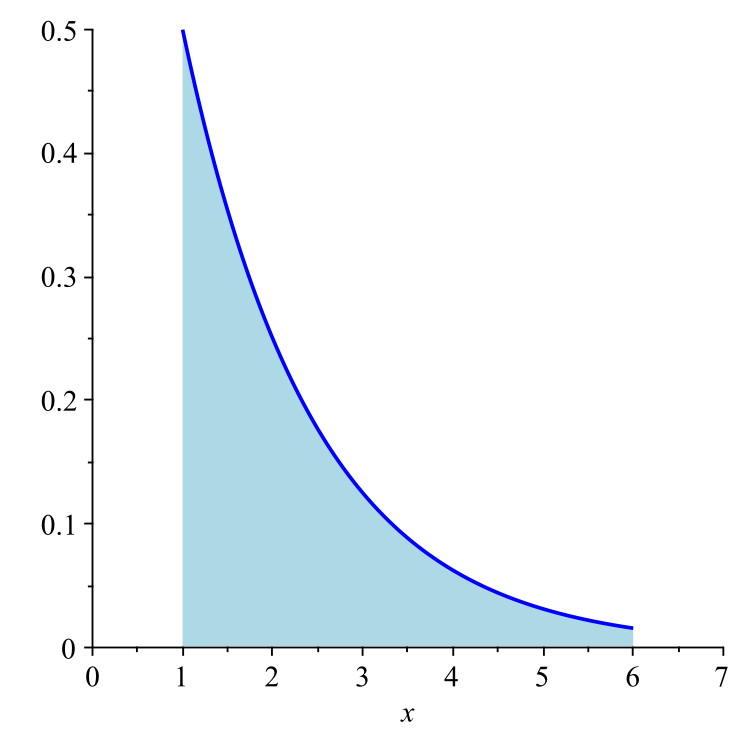
\includegraphics{1_b_area.eps}}
\end{center}
\caption{A region whose area we want to approximate.}
\label{F:1_b_area}
\end{figure}

Archimedes approached the problem of calculating the area of a quadratic region in the following way. Given a quadratic $q(x)$ on an interval $[a,b]$, Archimedes drew in a base given by the secant line connecting the points $(a,q(a))$ and $(b,q(b))$ as illustrated at left in Figure \ref{F:1_b_Archimedes}. Then he found the point in the interval $[a,b]$ at which the tangent line to the curve is parallel to the secant line. Archimedes gave an argument using mechanics (based on balance points), and then another using geometry (through a method of exhaustion) to show that the area of the parabolic region is $\frac{4}{3}$ times the area of the triangle determined by the endpoints and the point of tangency as shown at right in Figure \ref{F:1_b_Archimedes}.
\begin{figure}[h]
\begin{center}
\resizebox{!}{2.0in}{\includegraphics{1_b_Archimedes_1.eps}} \hspace{0.5in} \resizebox{!}{2.0in}{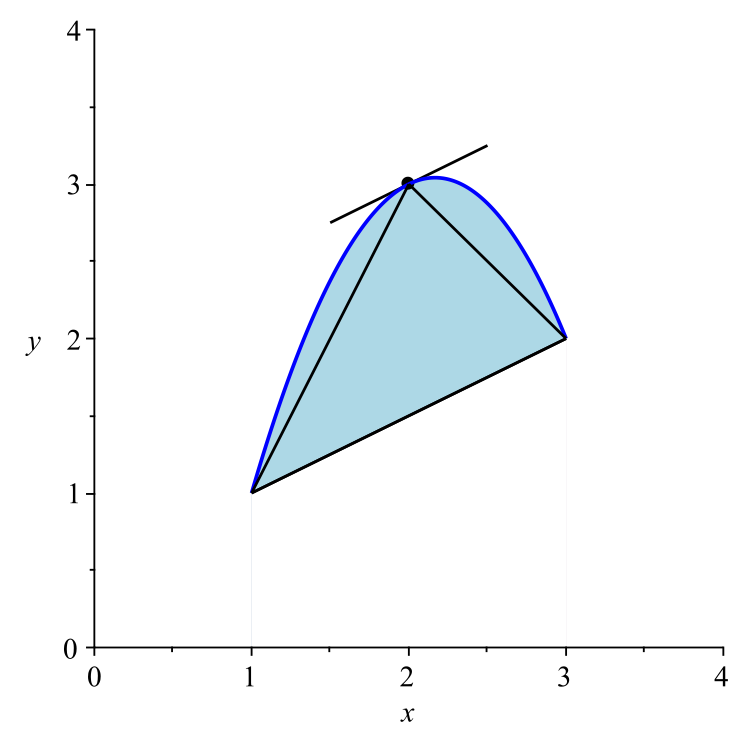
\includegraphics{1_b_Archimedes_2.eps}}
\end{center}
\caption{Archimedes method.}
\label{F:1_b_Archimedes}
\end{figure}
Although we won't go through the details, a conclusion we can draw from Archimedes argument, using the formula for the area of a rectangle and the area of a triangle, is that the area between the graph of a quadratic with equation $q(x) = ax^2+bx+c$ and the $x$-axis on an interval $[x_1, x_2]$ as illustrated in Figure \ref{F:1_b_quad_area} is 
\begin{equation} \label{eq:quad_area}
\frac{a}{3}(x_2^3-x_1^3) + \frac{b}{2}(x_2^2-x_1^2) + c(x_2-x_1).
\end{equation}
\begin{figure}[h]
\begin{center}
\resizebox{!}{2.5in}{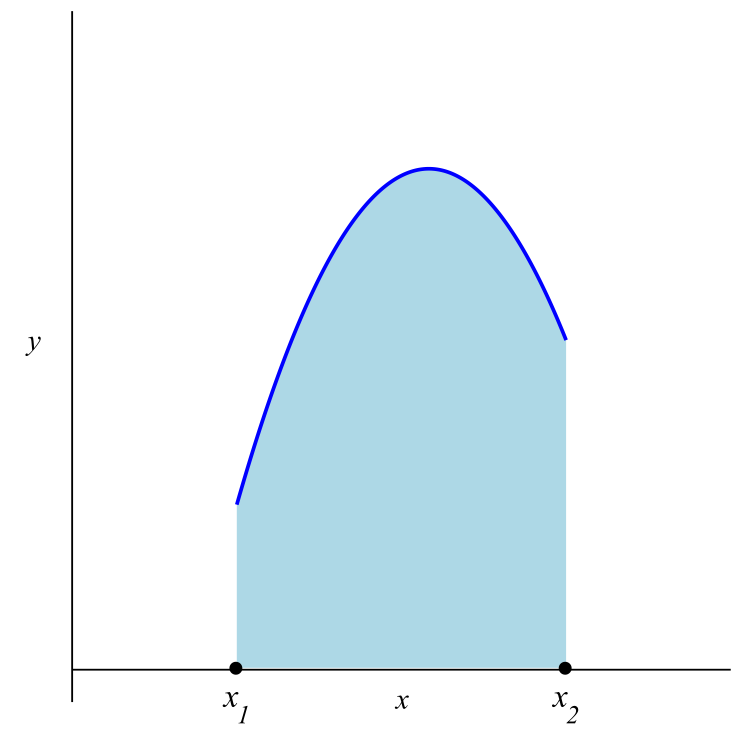
\includegraphics{1_b_quad_area.eps}} 
\end{center}
\caption{Region between a parabola and the $x$-axis.}
\label{F:1_b_quad_area}
\end{figure}
To approximate the area under the graph of a function, we will approximate the function itself with a collection of quadratics, and then use equation (\ref{eq:quad_area}) repeatedly. To do this, we need to know how to fit a quadratic curve to a three points. We consider that question now.

Suppose we are given a collection of three points in the plane: $(x_1, y_1), (x_2, y_2)$ and $(x_3, y_3)$. There is exactly one quadratic polynomial $p(x)$ which goes through these points, i.e. there is exactly one quadratic $p(x)$ such that for each $x_i$, $p(x_i)=y_i$. This is an example of \emph{polynomial curve fitting}\index{polynomial curve fitting}. 

As an example, we use the points $(-1, 2)$, $(1,6)$, $(2,5)$. To fit a quadratic to these points, consider a general quadratic of the form $p(x)=a_2x^2+a_1x+a_0$. By substituting the $x$ value of each of the given points and setting that equal to the $y$ value of that point, we find three equations
\[ (-1)^2a_2-a_1+a_0=2 \; , \; \quad a_2+a_1+a_0=6 \; , \; \quad (2)^2a_2 +2a_1+a_0=5 \]
that give us a system of three equations in the three unknowns $a_2$, $a_1$, and $a_0$:
\begin{alignat*}{4}
{}a_2	&{}-{} 	&{}a_1 	&{}+{}	&{}a_0 	&= 2   \\
{}a_2 	&{}+{}	&{}a_1 	&{}+{}	&{}a_0  &= 6   \\
{4}a_2	&{}+{} 	&{2}a_1	&{}+{} 	&{}a_0 	&= 5. 
\end{alignat*} 
This system is the example we considered in Preview Activity \ref{pa:1_b}, whose solution is $a_2 = -1$, $a_1=2$, and $a_0 = 5$. A graph of $q(x) = -x^2+2x+5$ along with the three points $(-1, 2)$, $(1,6)$, $(2,5)$ is shown in Figure \ref{F:1_b_quadratic_fit}. 
\begin{figure}[h]
\begin{center}
\resizebox{!}{2.5in}{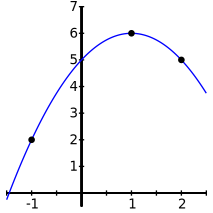
\includegraphics{1_b_quadratic_fit.eps}}
\end{center}
\caption{A quadratic fit to the points $(-1, 2)$, $(1,6)$, $(2,5)$.}
\label{F:1_b_quadratic_fit}
\end{figure}

Now that we know how to fit a quadratic to three points, we next approximate a curve with a collection of quadratics. The method we use is to break the interval on which our curve is defined into several subintervals and create quadratics on each subinterval. The basic idea is contained in our first project activity.
 
\begin{pactivity} \label{act:1_b_Simpson_ex_1}  In this activity we model the function $f$ defined by $f(x) = \sin(2x)+2$ on the interval $[a,b]$, where $a = -\frac{\pi}{2}$ and $b = \pi$ with a collection of quadratics. Let $f(x) = \sin(x)$. We divide the interval $[a,b]$ into three subintervals using the six points $x_0 = -\frac{\pi}{2}$, $x_1 = -\frac{\pi}{4}$, $x_2 = 0$, $x_3 = \frac{\pi}{4}$, $x_4 = \frac{\pi}{2}$, $x_5 = \frac{3 \pi}{4}$, and $x_6 = \pi$. We need three points to determine a quadratic, so the three subintervals of the interval $[a,b]$ will be the intervals $[x_0, x_2]$, $[x_2, x_4]$, and $[x_4,x_6]$. An illustration of the process of dividing our interval $[a,b]$ and approximating by quadratics can be found at \url{https://www.geogebra.org/m/spd4hhbw}. Round all calculations in this activity to the nearest thousandth.
	\ba
	\item Set up a system of linear equations to fit a quadratic $q_1(x) = r_1x^2+s_1x+t_1$ to the three points $(x_0, f(x_0))$, $(x_1, f(x_1))$, and $(x_2, f(x_2))$.  (The solution to this system to the nearest thousandth is $r_1 = 2$, $s_1 \approx 2.546$, and $t_1 = 1.621$.) 

	\item Set up a system of linear equations to fit a quadratic $q_2(x) = r_2x^2+s_2x+t_2$ to the three points $(x_2, f(x_2))$, $(x_3, f(x_3))$, and $(x_4, f(x_4))$. (The solution to this system to the nearest thousandth is $r_2 = 2$, $s_2 \approx  2.546$, and $t_2 \approx  -1.621$.)
	
	\item Set up a system of linear equations to fit a quadratic $q_3(x) = r_3x^2+s_3x+t_3$ to the 3 points $(x_4, f(x_4))$, $(x_5, f(x_5))$, and $(x_6, f(x_6))$. (The solution to this system to the nearest thousandth is $r_3 \approx 10.000$, $s_3 \approx  -7.639$, and $t_3 \approx  1.621$.)
	
	\item Use the GeoGebra applet at \url{https://www.geogebra.org/m/spd4hhbw} to graph the three quadratics on their intervals on the same axes as the graph of $f$. Explain what you see.

	\ea
\end{pactivity}  	

Project Activity \ref{act:1_b_Simpson_ex_1} illustrates how we can model a function on an interval using a sequence of quadratic functions. Now we apply this polynomial curve fitting technique to derive the general formula for approximating the area between a graph of a function $f$ and the $x$-axis. We use parabolic arcs to approximate the graph of $f$ on each subinterval. 

We start by dividing the interval $[a,b]$ over which our function is defined into some number of subintervals. We need an even number of subintervals, since we have to use three points to define each parabola. Let $n = 2m$ be the number of subintervals we use. In order to make the calculations a bit easier, let the subintervals all have the same length, which we denote by $\Delta x$ (the symbol $\Delta$ is often used in mathematics to indicate a change in a quantity). Since we have $n$ subintervals, the length of each subinterval will be $\Delta x = \frac{b-a}{n}$.  For each $k$ we let $x_k = a+k \Delta x$ and $y_k = f(x_k)$. Note that $x_0 = a$ and $x_n=b$. This labeling scheme is illustrated in Figure \ref{F:1_b_partition}
\begin{figure}[h]
\begin{center}
\resizebox{!}{2.5in}{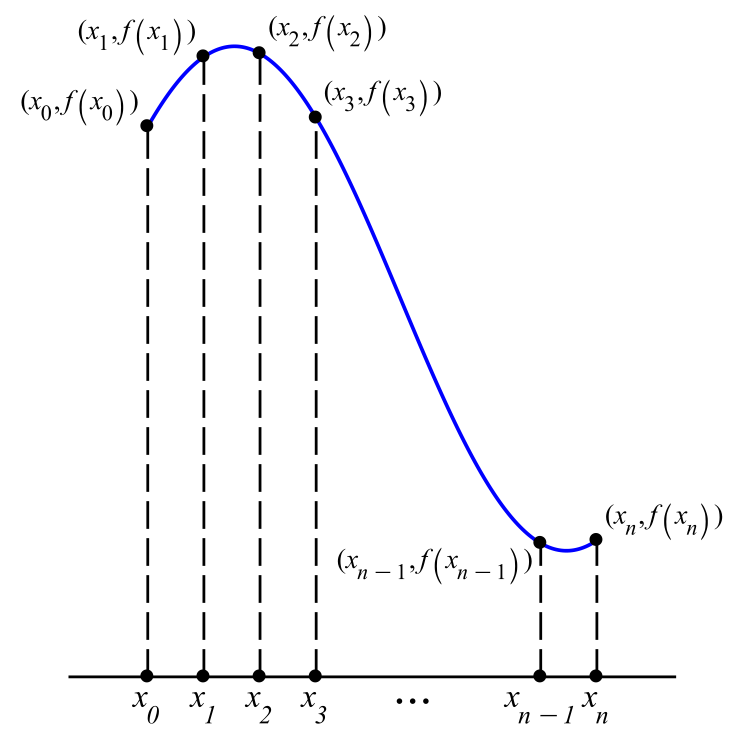
\includegraphics{1_b_partition.eps}}
\end{center}
\caption{Subdividing the interval $[a,b]$.}
\label{F:1_b_partition}
\end{figure}

We approximate $f$ on each subinterval using a quadratic. So we need to find the quadratic $Q(x) = c_2x^2+c_1x+c_0$ that passes through two consecutive end points as well as the midpoint of a subinterval. That is, we need to find the coefficients of $Q$ so that $Q$ passes through the points $(x_k,y_k)$, $(x_{k+2}, y_{k+2})$, and the midpoint $(x_{k+1},y_{k+1})$ on the interval $[x_k, x_{k+2}]$ (so that we have three points to which to fit a parabola) as shown at left in Figure \ref{F:1_b_quad_fit}. Note that the length of the interval $[x_k, x_{k+2}]$ is $2\Delta x$.  To make the calculations easier, we will translate our function so that our leftmost point is $(-r, y_k)$. Then the middle point is $(0, y_{k+1})$ and the rightmost point is $(r, y_{k+2})$ as illustrated at right in Figure \ref{F:1_b_quad_fit}, where $r = \Delta x$.   
\begin{figure}[h]
\begin{center}
\resizebox{!}{2.0in}{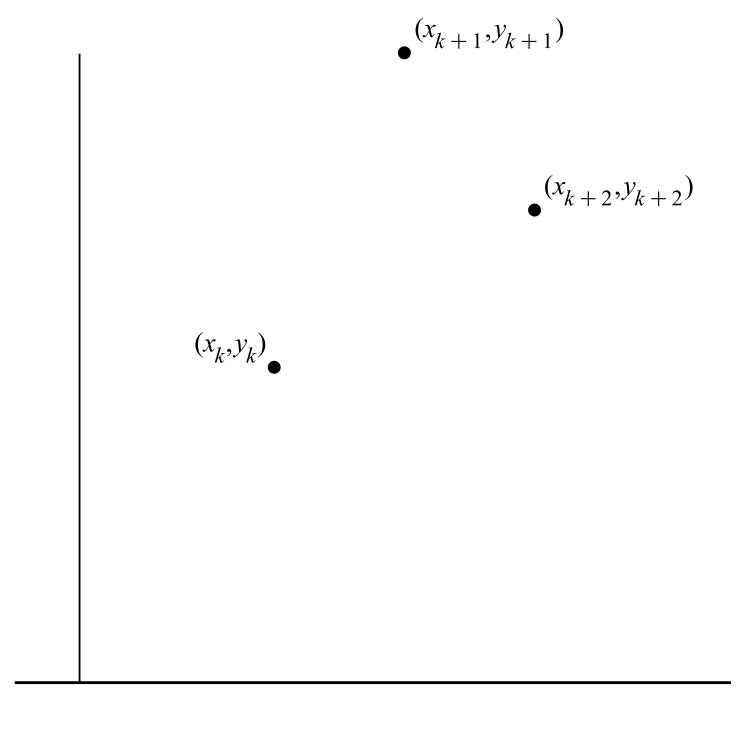
\includegraphics{1_b_quad_fit.eps}} \hspace{0.5in} \resizebox{!}{2.0in}{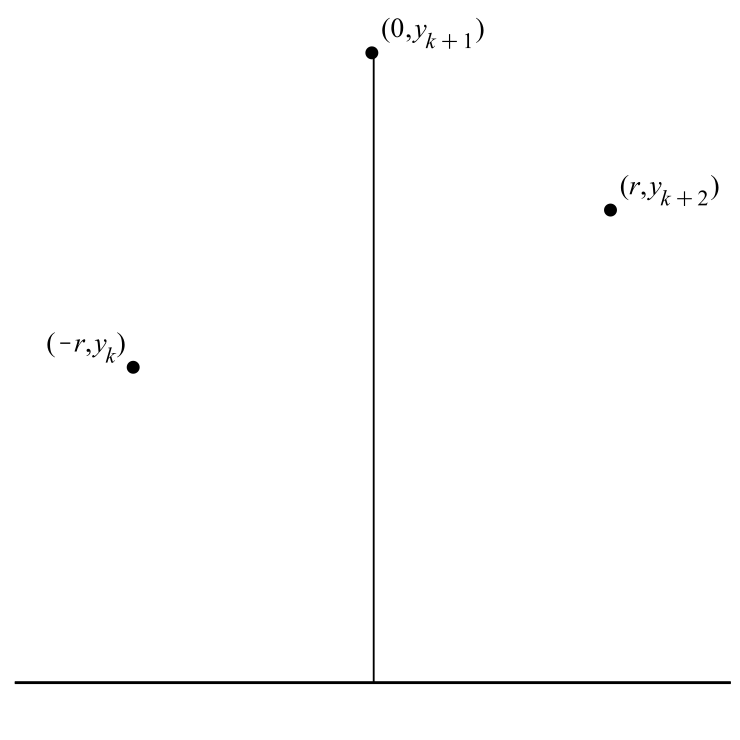
\includegraphics{1_b_translate.eps}}
\end{center}
\caption{Left: Three points. Right: Translated points.}
\label{F:1_b_quad_fit}
\end{figure}


\begin{pactivity} ~
	\ba
	\item Set up a linear system that will determine the coefficients $c_2$, $c_1$,  and $c_0$ so that the polynomial $Q(x) = c_2x^2+c_1x+c_0$ passes through the points $(-r, y_k)$, $(0, y_{k+1})$,  and $(r, y_{k+2})$ with $r \neq 0$. Remember that the unknowns in this system are $c_2$, $c_1$, and $c_0$. 

	\item Explain why the coefficient matrix of the system in part (a) is $\left[ \begin{array}{crc} r^2&-r&1 \\ 0&0&1 \\ r^2&r&1 \end{array} \right]$. Then explain why row reducing the matrix $\left[ \begin{array}{crcc} r^2&-r&1&y_k \\ 0&0&1&y_{k+1} \\ r^2&r&1&y_{k+2} \end{array} \right]$ will find the coefficients we want. Assume that a row echelon form of the matrix $\left[ \begin{array}{crcc} r^2&-r&1&y_k \\ 0&0&1&y_{k+1} \\ r^2&r&1&y_{k+2} \end{array} \right]$ is 
\[\left[ \begin{array}{crcc} r^2&-r&1&y_k \\ 0&2r&0&y_{k+2}-y_k \\ 0&0&1&y_{k+1} \end{array} \right].\]
Use these matrices to explain why $c_2=\frac{y_k-2y_{k+1}+y_{k+2}}{2r^2}$, $c_1=\frac{y_{k+2}-y_k}{2r}$, and $c_0 = y_{k+1}$. 

	\item Our goal is to ultimately approximate the area under the curve on the interval $[a,b]$ by approximating $f$ with quadratics on each subinterval. Use the Archimedean formula (\ref{eq:quad_area}) to show that the area under the quadratic $Q(x)$ from part (a) is 
\[\frac{1}{3}  \left(y_k+4y_{k+1}+y_{k+2}\right) \Delta x.\]

	\item Now add up all of the area approximations on each subinterval to show that the approximate area under the graph is given by the formula 
\begin{equation} \label{eq:1_b_Simpson_sum} 
S(n) = \left(y_0 + 4y_1 + 2y_2 + 4y_3 + 2y_4 + \cdots 2y_{n-2} + 4y_{n-1} + y_n\right) \frac{\Delta x}{3}.
\end{equation}


	\ea
	
\end{pactivity}

We conclude with an example.

\begin{pactivity} Let $f(x) = \left(\frac{1}{2}\right)^x$ on the interval $[1,6]$. A graph of $f$ is shown in Figure \ref{F:1_b_area}. Use our approximation formula with $n=8$ to approximate the area of the shaded region in Figure \ref{F:1_b_area}. Show all of your work and round all calculations to the nearest thousandth. 

\end{pactivity}



